\documentclass[border=6pt]{standalone}
\usepackage{tikz}
\usetikzlibrary{arrows.meta,positioning}
\begin{document}
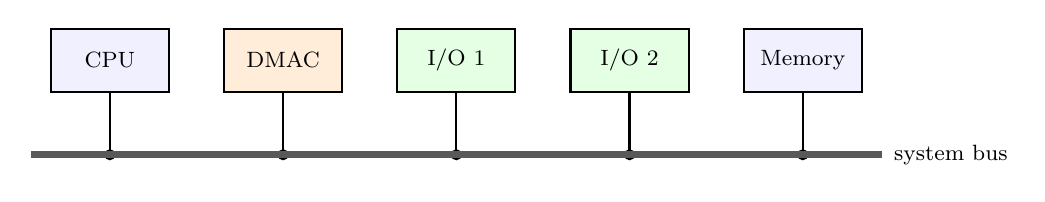
\begin{tikzpicture}[font=\small,
 m/.style={draw,thick,fill=blue!6,minimum width=1.5cm,minimum height=0.8cm,align=center,font=\footnotesize}]
\foreach \x/\n/\c in {0/CPU/blue!6,2.2/DMAC/orange!15,4.4/I\slash O 1/green!10,6.6/I\slash O 2/green!10,8.8/Memory/blue!6} {
  \node[m,fill=\c] at (\x,0) {\n};
  \draw[thick] (\x,-0.4) -- (\x,-1.2);
  \fill (\x,-1.2) circle (2pt);
}
\draw[line width=2.5pt,gray!70!black] (-1.0,-1.2) -- (9.8,-1.2) node[right,font=\footnotesize,black]{system bus};
\end{tikzpicture}
\end{document}
